\documentclass{beamer}
\usepackage[utf8]{inputenc}
\usepackage{hyperref}
\usepackage{forloop}
\usepackage{amsmath,amsfonts,amssymb}
\useoutertheme {smoothbars}

\usepackage{listings}
\usepackage{color}
\definecolor{name}{rgb}{0.5,0.5,0.5}
\definecolor{javared}{rgb}{0.6,0,0} % for strings
\definecolor{javagreen}{rgb}{0.25,0.5,0.35} % comments
\definecolor{javapurple}{rgb}{0.5,0,0.35} % keywords
\definecolor{javadocblue}{rgb}{0.25,0.35,0.75} % javadoc
\lstset{language=Java,
	basicstyle=\ttfamily,
	keywordstyle=\color{javapurple}\bfseries,
	stringstyle=\color{javared},
	commentstyle=\color{javagreen},
	morecomment=[s][\color{javadocblue}]{/**}{*/},
	numbers=left,
	numberstyle=\tiny\color{black},
	stepnumber=2,
	numbersep=10pt,
	tabsize=4,
	showspaces=false,
	showstringspaces=false}
\defbeamertemplate*{footline}{smoothbars theme}
{%
	\begin{beamercolorbox}[colsep=1.5pt]{upper separation line foot}
	\end{beamercolorbox}
	\begin{beamercolorbox}[ht=6ex,dp=1.125ex,%
		leftskip=.3cm,rightskip=.3cm plus1fil]{title in head/foot}%
		\leavevmode{\usebeamerfont{title in head/foot}\insertshorttitle}%
		\hfill%
		{\usebeamerfont{author in head/foot}\usebeamercolor[fg]{author in head/foot}\insertshortauthor}
		\vspace{.8mm}
		
		\url{http://creativecommons.org/licenses/by-nd/4.0/}%
	\end{beamercolorbox}%
	\begin{beamercolorbox}[colsep=1.5pt]{lower separation line foot}
	\end{beamercolorbox}
}
\author[Janis Streib]{Janis Streib \\ CC-BY-ND-4.0} 


\begin{document}
%\def\pause{}
\title{RESTaurant for Android: Programmierung einer Sitzplatzreservierung \\ Teil III}   

\date{02.-06.11.2015}

\frame{\titlepage}

\frame{\frametitle{Inhalt}\tableofcontents} 

%\lstinputlisting{filename.java}
%\begin{lstlisting}
% Add code here
%\end{lstlisting}
\section{Exkurs: XML}
\subsection{XML}
\frame{\frametitle{Exkurs: XML}
	\begin{itemize}
		\item XML := Extensible Markup Language
		\item Erweiterbare Auszeichnungssprache zur Auszeichnung hierarchischer Strukturen
	\end{itemize}
}

\section{UI}
\subsection{Übersicht}
\frame{\frametitle{Das Android UI}
	\begin{columns}
		\begin{column}{.62\textwidth}
			\begin{enumerate}
				\item \emph{Actionbar}
				\item \emph{Optionmenu}
				\item \emph{Statusbar}
				\item \emph{Toast}
			\end{enumerate}
			Das ganze "Fenster" (mitsamt Logik dahinter), wie es hier Vorliegt: \\ \emph{Activity}
				\begin{itemize}
					\item Beschriebung erfolgt in XML-Dateien
				\end{itemize}
		\end{column}
		
		\begin{column}{.38\textwidth}
		%	\begin{picture}(2,2)
		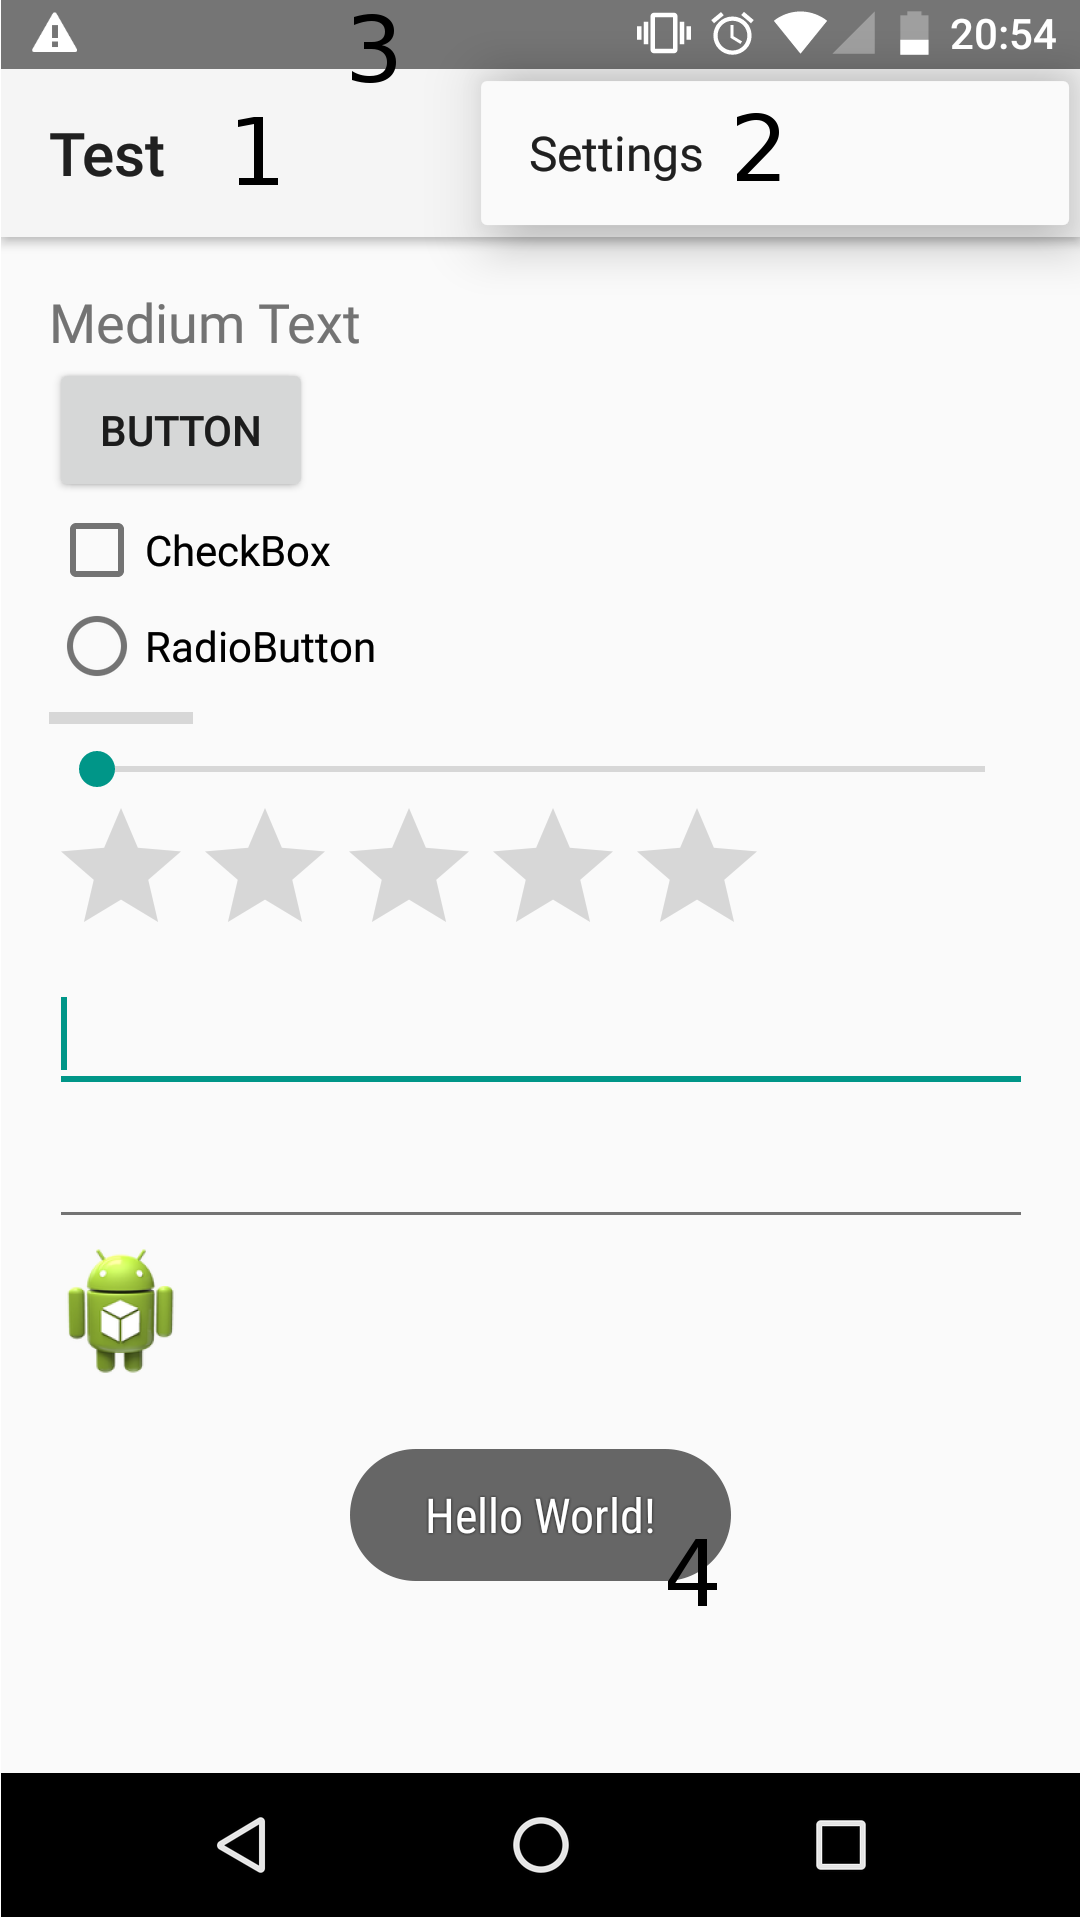
\includegraphics[width=36mm]{img/ui}
		%	\end{picture}
			%\includegraphics[\textwidth]{fig}
		\end{column}
	\end{columns}
}

\subsection{Beschreibung}
\frame{\frametitle{Die Beschreibung des Android UIs}
	\begin{columns}
		\begin{column}{.67\textwidth}
				\tiny {\lstinputlisting[language=XML]{samples/ui2.xml}}
		\end{column}
		
		\begin{column}{.33\textwidth}
			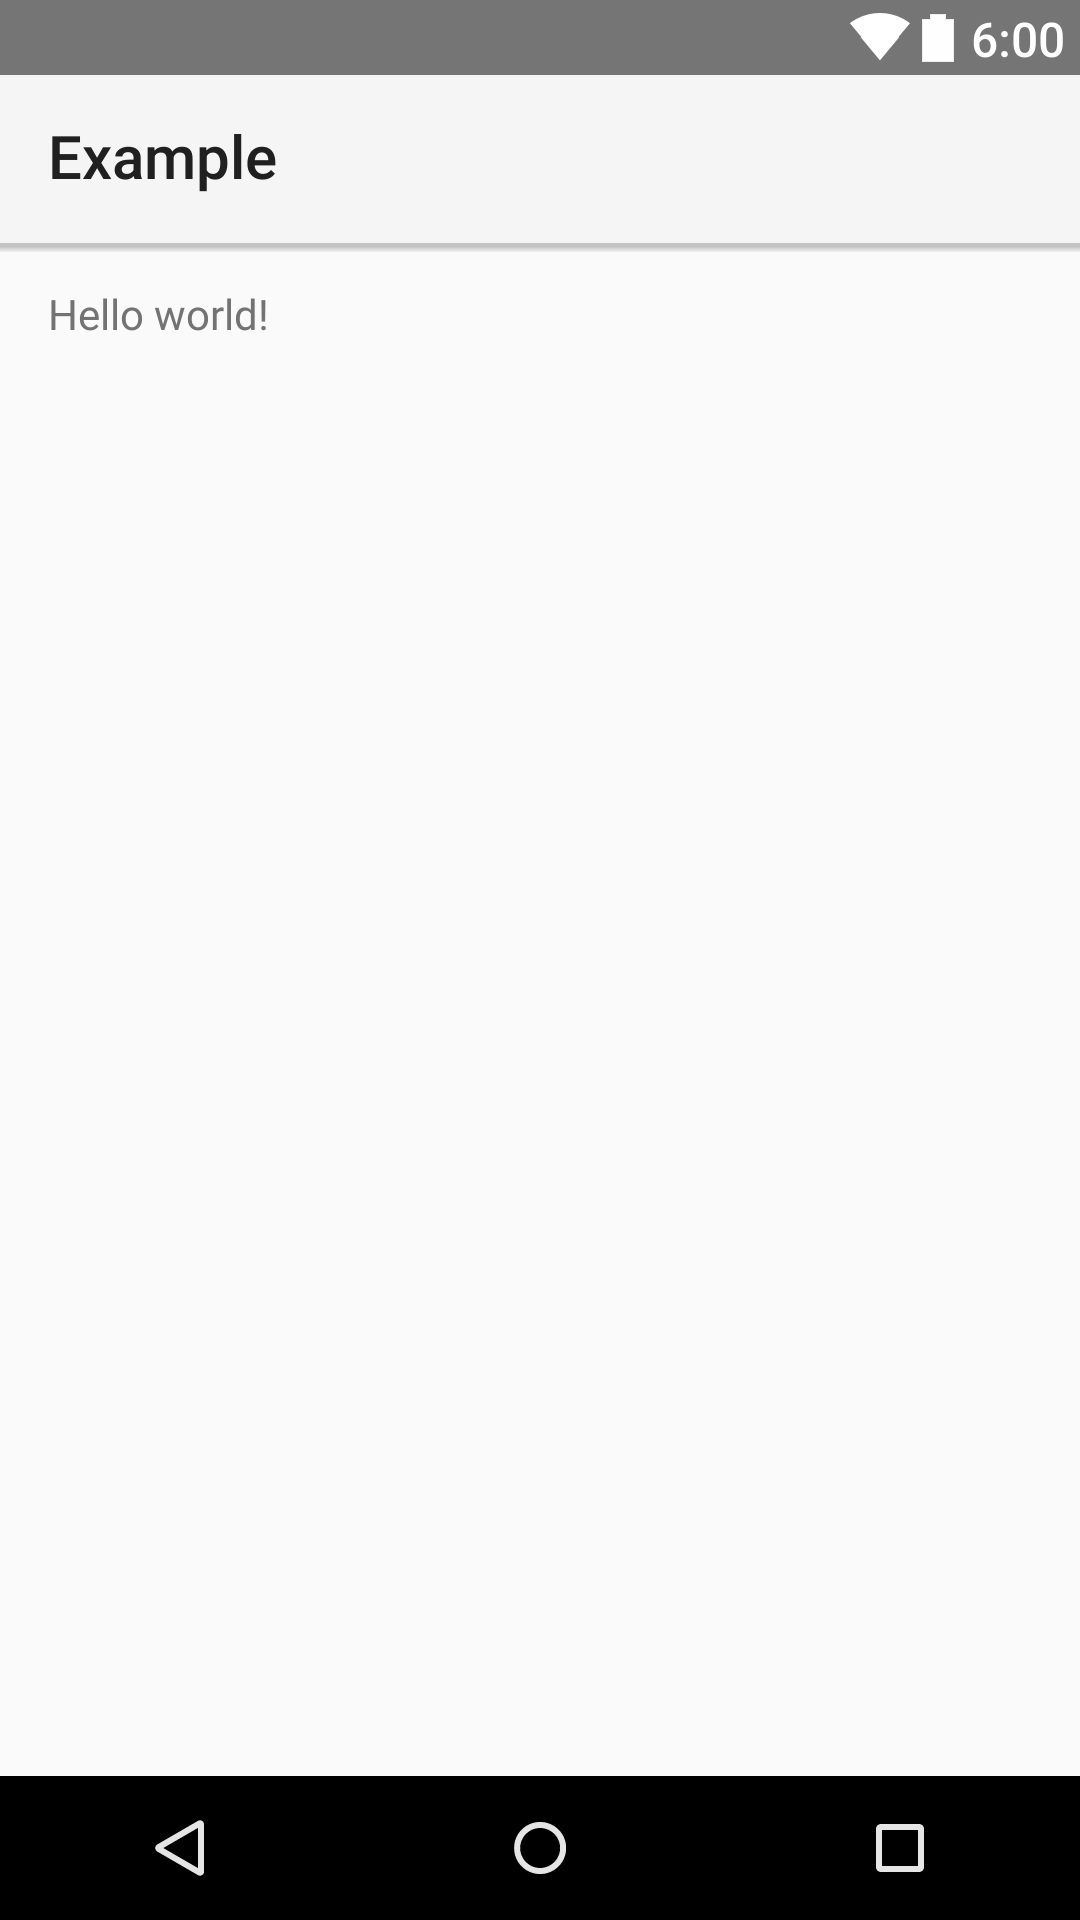
\includegraphics[width=36mm]{img/ui2}
		\end{column}
	\end{columns}
}
\frame{\frametitle{Die Beschreibung des Android UIs}
	\begin{columns}	
		\begin{column}{.67\textwidth}
			\tiny {\lstinputlisting{samples/ui3.xml}}
		\end{column}
		
		\begin{column}{.33\textwidth}
			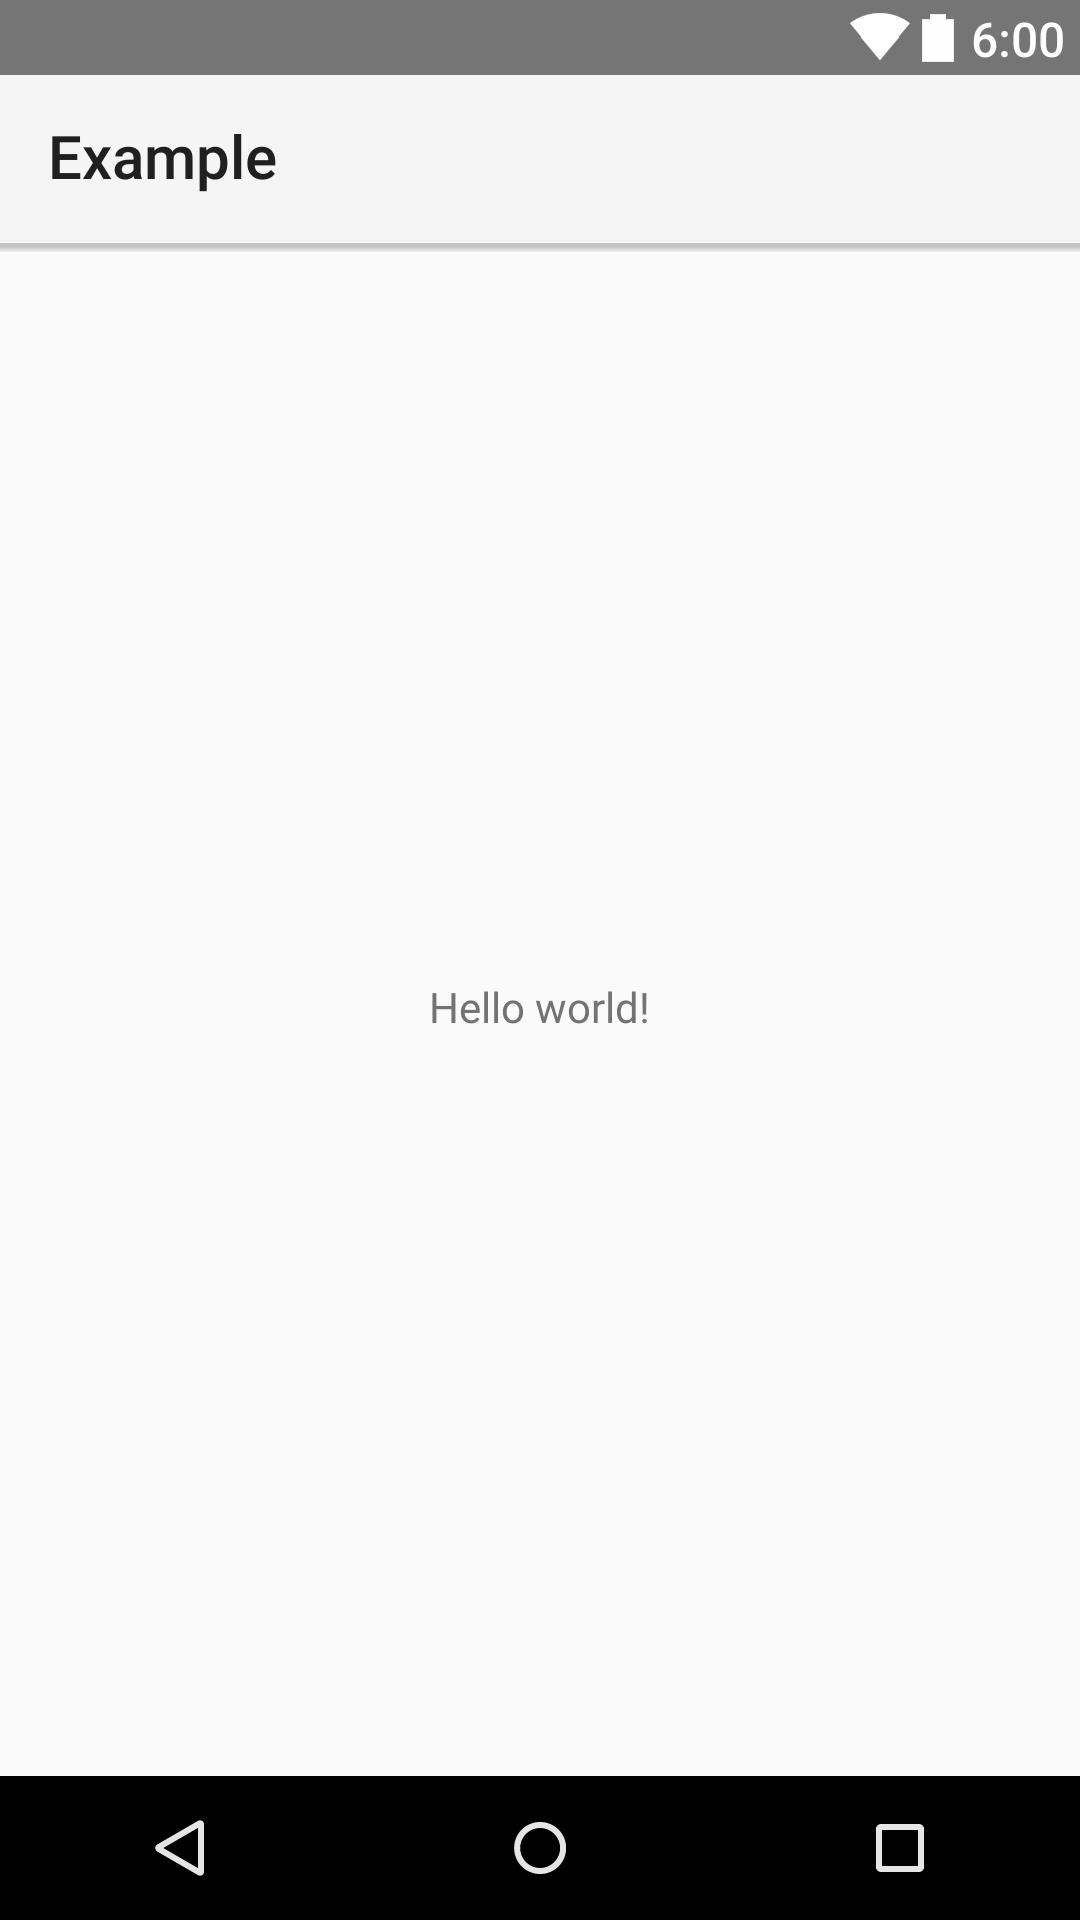
\includegraphics[width=36mm]{img/ui3}
		\end{column}
	\end{columns}
}
\section{UI-Gestaltung}
\forloop{ct}{1}{\value{ct} < 9}%
{%
	\frame{\frametitle{Ein esrtes UI gestalten}		
		\includegraphics[width=116mm]{img/new\arabic{ct}}
	}
}
\section{UI zu Code}
\subsection{Von Android Studio zu NetBeans}
\forloop{ct}{1}{\value{ct} < 6}%
{%
	\frame{\frametitle{Von Android Studio zu NetBeans}		
		\includegraphics[width=116mm]{img/a2n\arabic{ct}}
	}
}
\frame{\frametitle{Vom UI zum Code}
	\begin{itemize}
		\item Jedes UI-Element in Android ist von der Grundklasse ein {\tt View}
		\item Alle UI-Elemente, denen im XML-File eine Id ({\tt android:id=""}) gegeben wurden, werden in Java von der IDE in die Klasse {\tt R} abgebildet
		\item Im Code können die Views dann über {\tt findViewById(R.id.\{viewId\})} referenziert werden
		\item Referenzierung als Button, TextView, usw. der Views im Code durch Casts 
	\end{itemize}
}
\section{Zinsrechner}
\frame{\frametitle{Mini-Projekt: Zinsrechner}
	Designen und Bauen Sie einen kleinen Zinsrechner, bei dem der Benutzer ein Startkapital und einen Zinssatz angeben kann und sein Endkapital zurückgeliefert bekommt.
	
	\pause Musterlösung:\\ \url{https://github.com/janisstreib/RESTaurant/tree/master/Zinsrechner}
}
\section{Zustandshaltung}
\frame{\frametitle{Zustandshaltung}
	\begin{itemize}
		\item Experiment mit dem Zinsrechner: Display drehen (in einem AVD: {\tt Strg + F11} / {\tt Strg + F12}) \pause
		\item Grund: Bei jedem komplett neuen Zeichnen des UIs wird {\tt onCreate()} neu aufgerufen und die Activity neu instanziiert \pause
		\item Lösung: {\tt onSaveInstanceState()} und {\tt onRestoreInstanceState()} sowie der Parameter {\tt savedInstanceState} in {\tt onCreate()}
		\item Variablen und Zustände werden in einem {\tt Bundles} bei {\tt onRestoreInstanceState()} gespeichert und vom Android-System entgegengenommen. Wenn die Activity vom System wieder geweckt wird, wird dieses Bundle der Activity wieder zurückgeführt.
		\item $\Rightarrow$ Android-System kann auch aus anderen Gründen die Activity "killen"
	\end{itemize}
}
\frame{\frametitle{Beispiel}
	\tiny{ \lstinputlisting{samples/Instance.java} }
}
\frame{\frametitle{Implementieren}
	Implementieren Sie die Zustandshaltung in Ihrem Zinsrechner.\\
	Musterlösung: \\\pause
	\url{https://github.com/janisstreib/RESTaurant/tree/master/ZinsrechnerEnhanced}
}
\section{Android Documentaion}
\frame{\frametitle{Android Documentation}
	\begin{itemize}
		\item Aktuelle Guidelines, Tutorials, Dokumentation: \\ \url{https://developer.android.com}
	\end{itemize}
}
%\section{Teil IV: Android UI-Design}
%\section{Teil V: Das RESTAurant}
%\section{Optional: Teil VI: Android Design Guidelines}
%\section{Optional: Teil VII: Versionskontrolle}
\end{document}

